% https://github.com/martinhelso/MathDept


\documentclass[UKenglish]{beamer}

\usetheme[NoLogo]{MathDept}

\usepackage[utf8]{inputenx} % For æ, ø, å
\usepackage{babel}          % Automatic translations
\usepackage{csquotes}       % Quotation marks
\usepackage{microtype}      % Improved typography
\usepackage{amssymb}        % Mathematical symbols
\usepackage{mathtools}      % Mathematical symbols
\usepackage[absolute, overlay]{textpos} % Arbitrary placement
\setlength{\TPHorizModule}{\paperwidth} % Textpos units
\setlength{\TPVertModule}{\paperheight} % Textpos units
\usepackage{tikz}
\usepackage{diagbox}
\usetikzlibrary{overlay-beamer-styles}  % Overlay effects for TikZ

% Extra 
\usepackage{siunitx}


\author[Mikkel Metzsch Jensen]{Mikkel Metzsch Jensen}
\title[Predicting Graphene Kirigami Friction]{Predicting Frictional Properties of Graphene Kirigami Using Molecular Dynamics and Neural Networks}
\subtitle{Designs for a negative friction coefficient} 
\institute[UiO]{University of Oslo}
\date[Juni 02, 2023]{Juni 02, 2023}

\begin{document}



\begin{frame}{Outline}
    \tableofcontents
\end{frame}


\section{Introduction} %%%%%%%%%%%%%%%%%%%%%%%%%%%%%%%%%%%%%%%%%%%%%%%%%%%%%%%%%%%%%
\subsection{Thesis overview}

\begin{frame}[c]
	\frametitle{Overview}
	\framesubtitle{Three main parts}
	
	\begin{enumerate}
		\setlength\itemsep{1em}
		\item \textbf{Sheet kirigami}: Alter a graphene sheet using atomic scale cuts and stretching
		\item \textbf{Forward simulation}: Calculate the frictional properties of the sheet using MD simulations
		\item \textbf{Accelerated search}: Use machine learning to replace the MD simulations and perform an accelerated search for new designs
	\end{enumerate}
	\vspace{2mm}
	
	Can we control the frictional properties of a graphene sheet using this technique?
	% \begin{itemize}
	% 	\item Can we utilize a coupling between load and stretch?
	% 	\item Negative friction coefficients
	% \end{itemize}
	
\end{frame}


\subsection{Motivation}


\begin{frame}
	\frametitle{Motivation}

	\begin{itemize}
		\item Kirigami: Variation of origami with cuts permitted
		\item Macroscale designs $\to$ nanoscale
	\end{itemize}
	\vspace*{10px}

	\begin{figure}
		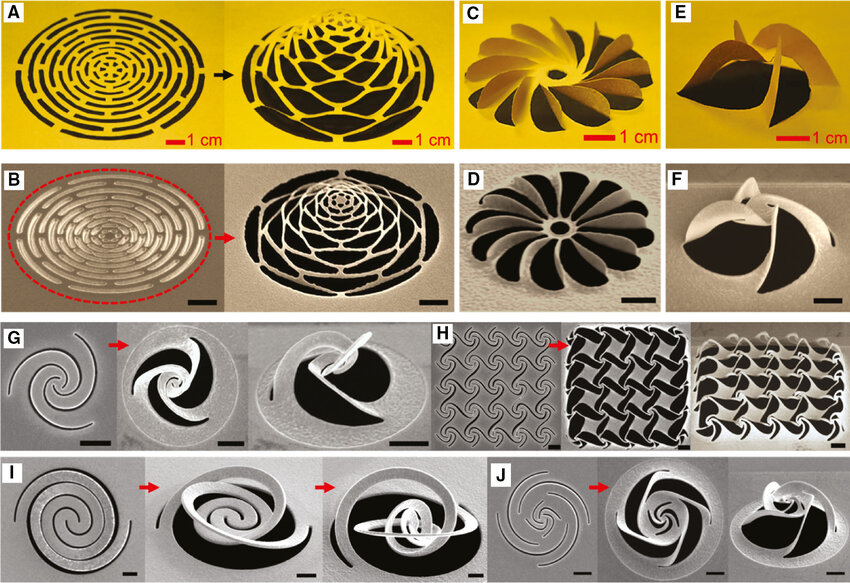
\includegraphics[height=0.6\textheight]{figures/kirigami_example.jpg}
		\caption{Example of macroscale Kirigami designs implemented on a nanoscale using a focused ion-beam (FIB). Black scale bars: \SI{1}{\mu m}. Reproduced from \cite{Li_2018}.}
	\end{figure}	

\end{frame}

\section{Creating a graphene Kirigami system} %%%%%%%%%%%%%%%%%%%%%%%%%%%%%%%%%%%%%%%%%%%%%%%%%%%%%%%%%%%%%
\subsection{System setup}
\subsection{Kirigami}




\section{Pilot study} %%%%%%%%%%%%%%%%%%%%%%%%%%%%%%%%%%%%%%%%%%%%%%%%%%%%%%%%%%%%%
\subsection{Friction metrics}
\subsection{Out-of-plane buckling}
\subsection{Friction-strain profiles}
\subsection{Negative friction coefficient}


\section{Kirigami configuration search} %%%%%%%%%%%%%%%%%%%%%%%%%%%%%%%%%%%%%%%%%%%%%%%%%%%%%%%%%%%%%
\subsection{Machine learning}
\subsection{Accelerated search}



\section{Summary and outlook} %%%%%%%%%%%%%%%%%%%%%%%%%%%%%%%%%%%%%%%%%%%%%%%%%%%%%%%%%%%%%



\begin{frame}%[allowframebreaks]
	\frametitle{References}
	\bibliographystyle{apalike}
	\bibliography{./bibliography.bib}
\end{frame}


\end{document}